\chapter{Baselines, ablations, and cost-accuracy tradeoffs}
\label{ch02-baselines-ablations-cost-accuracy}
In one end-to-end run of CodeProbe (\href{https://github.com/sjarmak/codeprobe}{public repository}), the plain baseline came out ahead of the tool-augmented arm on both score and score per dollar. The configuration with the retrieval machinery in it lost to the configuration with none. That outcome was visible only because the run included a baseline at all. Reported alone, the tool arm's score would have had nothing to be read against, and a reader could have credited the retrieval machinery with whatever the number implied.

Published comparisons frequently omit the inexpensive arm. Kapoor et al.~(\href{https://arxiv.org/abs/2407.01502}{2024}) re-evaluated published agent architectures and found that on HumanEval, retrying the model could match more elaborate architectures at a fraction of their inference cost. When they optimized cost and accuracy jointly, they reduced cost without giving up accuracy.

Those results do not establish the same conclusion for repository-scale engineering. The re-evaluation is directional, and its coding evidence comes from a function-level benchmark. The comparison design transfers even when the finding does not. The inexpensive arm belongs in the experiment, and cost belongs in the report.

That omission changes the claim. A system with memory, retrieval, tools, or multiple agents may score higher than a direct model call. The score alone cannot tell us whether the added machinery caused the gain, whether another model call would have produced the same gain, or whether the comparison spent more until it found more successful samples. Engineering selection requires two coordinates: what the system accomplishes and what it consumes.

The available evidence supports comparison design rather than a universal cost threshold or recommended architecture. The chapter therefore develops controls that readers can run on their own workloads.

An elaborate system is worth keeping only when both comparisons support it. Its components must contribute something that remains when the rest of the experiment is held fixed, and the full configuration must beat the simple alternatives at a cost the operator is willing to pay. These are separate tests. Component removal addresses causal attribution. Direct-call and retry baselines address engineering value.

\hypertarget{remove-the-component-and-rerun-the-evaluation}{%
\section{Remove the component and rerun the evaluation}\label{remove-the-component-and-rerun-the-evaluation}}

An \textbf{ablation} removes one component and reruns the evaluation with the rest of the system and procedure held fixed. If a memory-enabled agent outperforms an agent without memory, the missing-memory arm estimates what the memory system contributed. If the comparison changes the model, prompt, task subset, token budget, harness version, or scoring procedure at the same time, the subtraction no longer isolates memory. It measures an unspecified bundle of changes. Without the missing-component arm, base-model capability and item difficulty remain plausible explanations for the observed score.

The component controls recur in two source corpora. SkillEvolBench, from Lei et al.~(\href{https://arxiv.org/abs/2605.24117}{2026}), reports no-skill and raw-trajectory controls for agent memory. CoIR, from Li et al.~(\href{https://arxiv.org/abs/2407.02883}{2024}), supplies the task and metric substrate for code retrieval, while the no-tool control comes from the associated evaluation-design synthesis. These sources support narrower measurements in their own settings; neither tests the complete repository-scale prescription developed here. Their convergence motivates the protocol, while the generalized recommendation remains directional.

Memory requires at least three arms. The first is the proposed memory system. The second is the no-skill control, which removes the written memory entirely. The third reuses the raw trajectory from prior work without asking a writer to consolidate it into a skill or memory record. The no-skill arm tests whether prior experience helps at all. The raw-trajectory arm tests whether the consolidation mechanism adds anything beyond retaining the original evidence.

Those two questions are easy to collapse into one. Suppose an agent that receives a distilled lesson solves more tasks than an agent starting from an empty context. The gain could come from the lesson, but it could also come from any useful tokens copied out of the earlier attempt. Raw-trajectory reuse makes that alternative visible. If the raw trace matches the distilled record, the experiment has shown that prior information helps, but it has not shown that the writer extracted a better representation.

The comparison also needs matched opportunities to retrieve. A memory arm evaluated on tasks for which a relevant record exists cannot be compared directly against a no-memory arm scored across a broader or harder task set. The primary comparison should be restricted to a coverage-matched subset, that is, the tasks for which the memory or retrieval system had a genuine opportunity to return relevant material. The full-set result should be reported separately, because coverage is itself an operational property. Unequal coverage should not be read as a difference in answer quality.

Retrieval and tool evaluations need a corresponding no-tool arm. Tool availability is an experimental variable and should be recorded with the rest of the arm configuration. The control gets the same base model, instructions, stopping conditions, and task instances, with access to the tool removed. If the treatment also receives a different system prompt, a larger context budget, or extra retries, those changes belong in additional arms or in a sweep that varies them one at a time.

One-factor sweeps matter because agent components interact. Retrieval can change context length. Context length can change model behavior. Tool schemas consume tokens before the agent begins the task. A different endpoint can expose a different tool set. A single comparison between `agent' and `baseline' assigns the combined effect to whichever feature appears in the label. Factorial experiments can estimate interactions when the evaluation budget supports them, but a sequence of one-factor comparisons is usually enough to find the first unsupported attribution.

An ablation result is conditional on the configuration in which the removal occurred. If retrieval helps only when a summarizer compresses its output, removing retrieval from the full system estimates retrieval's contribution with that summarizer present. The result does not show whether retrieval would help without summarization, or whether summarization would help without retrieval. Those questions require the corresponding component combinations as separate arms.

Skills and multi-agent structures need the same discipline, but their removal needs a more precise intervention. Deleting a skill while also shortening the prompt changes both procedural guidance and context length. Replacing several agents with one while reducing the call budget changes topology and sampling opportunity together. A useful control preserves the available information and budget wherever the design permits and removes only the coordination or representation being credited. When that preservation is impossible, an intermediate arm lets the comparison separate fewer model calls from a different arrangement of those calls.

Tank and Nama (\href{https://arxiv.org/abs/2607.22520}{2026}) compared agents with and without procedural skills across nearly 6,000 runs on two office-automation benchmarks and three model-harness stacks. The best-performing skills won primarily by causing fewer regressions, a distinction concealed by net task-success change. The study strongly supports decomposing a skill intervention into gains, regressions, and residual failures in those settings; transfer to coding-agent skill libraries remains directional.

The paired design from Chapter 1 belongs here. Each arm runs on the same tasks, task ordering and other sources of randomness are matched across arms wherever the execution system permits it, and the outcomes are analyzed as pairs. Otherwise, item difficulty can dominate the component effect. A retrieval arm that happens to receive more questions answerable by lexical lookup may appear superior even when the tool adds nothing on matched items.

Target size is a second confound of the same kind. A tool may look better when its index contains a narrow, curated collection and worse when it searches a large repository with many plausible distractors. Query coverage, corpus size, and retrieval depth should therefore be recorded with the configuration. If target size changes between arms, the experiment measures both the target and the retrieval algorithm.

In two studies from my own team, we asked the same practical question: does a retrieval tool help an agent? The positive-sign study was a paired comparison across many repositories, in which the tool arm came out slightly ahead. The negative-sign study was the CodeProbe run described at the start of this chapter, in which the plain baseline came out ahead. The two used different task curation and different enforcement of which arm had to use the capability under test. That experience is narrative illustration rather than independent evidence for the control method, but it exposed the mechanism. The apparatus decided which work entered the evaluation and whether the agent had to use the capability supposedly under test. The label on the treatment arm therefore did not identify a stable intervention.

Arm separation should be established at the task level through observed usage. A task cannot estimate a tool effect when the treatment completes it without touching the tool. Such a task may remain useful for measuring the agent's overall capability, but it contributes no information to the comparison of tool access.

In my own enterprise-scale benchmark, one candidate task ran for 41 turns without a single call to the tool under test. By every static check we had, it was a perfect task, and for the tool comparison it was useless. We removed it from the tool-effect comparison because both arms had effectively received the same treatment. Candidate tasks are hypotheses about discrimination, and a pilot run has to show that they actually separate the arms.

This gate should be empirical. For every candidate task, record whether the treatment invoked the component, whether the control could reach it through another path, and whether both arms received equivalent task information. A binary `tool enabled' field is inadequate when the agent may ignore the tool. Usage counts, arguments, returned bytes or tokens, and the point in the trajectory where the result entered context make the intervention observable.

The exclusion rule needs the same protection as any other post-hoc filter. Removal should be keyed to observed component usage and declared before the outcomes are inspected. Dropping tasks after seeing which arm won selects on the result, and it converts a usage gate into a mechanism for improving the reported effect.

Usage does not establish usefulness, but absence establishes non-use. If the treatment calls a retriever and then ignores its output, the task may still show a cost effect or an interference effect. If it never calls the retriever, its outcome cannot support a claim about retrieved information improving correctness.

The strongest boundary concerns information flow into the component. Evaluation labels and gold answers must stay out of any memory writer. A writer that sees the correct answer can encode it directly, encode a near paraphrase, or preserve features that make later retrieval trivial. Freezing the memory after that write does not repair the experiment, because the evaluated artifact already contains the target.

The same rule applies to the scoring target. A `right answer' generated with the tool or mechanism under evaluation cannot then be used to grade that mechanism by agreement with its own output. A retrieval system compared against answers assembled from the same retrieval system has been graded against its own oracle, the reference an evaluation scores candidate answers against. A target capable of disagreeing with the system requires independent human verification, or sources outside the evaluated path. Public benchmarks carry a related problem, because models have often already seen those tasks during training, an inflation channel Chapter 3 measures.

An ablation cannot remove every threat to inference, and it does not show that a useful component will remain useful under another workload. It answers a narrower question: under the evaluated task distribution and the fixed surrounding system, did removing this component change the measured outcomes? This question is narrow enough to test and strong enough to prevent a common attribution error.

The completed record should make the subtraction reproducible. Name the component removed, list every configuration field that remained fixed, identify the coverage-matched task subset, report component usage per task, and preserve the paired results. When multiple factors changed, describe the arm as a bundle and resist assigning its effect to one member of that bundle.

\hypertarget{select-on-accuracy-and-cost-together}{%
\section{Select on accuracy and cost together}\label{select-on-accuracy-and-cost-together}}

The support for this entry is one directional re-evaluation study and no strong evidence item. Kapoor et al.~(2024) covered a small set of benchmark families, including function-level coding, multi-hop question answering, and web-agent tasks. They did not establish the same result for repository-scale software work. Their contribution here is a comparison design that can be applied beyond those tasks. Evaluate the elaborate system against direct model calls and retries, then place accuracy and inference cost in the same result.

Additional model calls can raise the pass rate without any change to the architecture. If one attempt has probability \(p\) of passing and two attempts are independent, the probability that at least one passes is \(1-(1-p)^2\). The expression illustrates the effect under independence. It does not estimate real agent behavior, in which attempts are correlated. Correlation changes the size of the gain, but a system allowed to sample, revise, or delegate more often still has more opportunities to produce a passing output.

An accuracy-only ranking conceals those opportunities. It may rank a five-call scaffold above a direct call without showing that the improvement came from four additional samples. It may also compare one architecture with a retry loop against another configured to stop after its first answer. The ranking then credits budget and stopping policy under the name of architecture.

Use at least three initial arms. The direct-call arm sends the task to the base model with the minimum production-valid prompt and no scaffold. The retry-once arm makes one additional model attempt after a defined failure signal. The candidate arm runs the proposed architecture with its intended tools, memory, or delegation.

The failure signal in the retry arm must be available to the deployed system. Unit tests, a compiler error, or a schema validator can supply one. A hidden benchmark answer cannot. If the experiment retries only because the evaluator knows the first answer is wrong, that arm should be labeled oracle-assisted, because it otherwise understates the operational cost of deciding when to retry.

Model version, task set, and scoring target stay fixed across the three arms. Match any shared context required to attempt the task, but do not give the direct call internal traces that exist only because the scaffold ran. The inexpensive alternative has to be built credibly, since a deliberately crippled direct call provides no useful control. Record the stopping condition for every arm, because `one run' can mean one model response, one agent trajectory, or a tree of dozens of calls.

Cost accounting begins at the task boundary. Count all input and output tokens consumed after the task enters the system, including calls made by planners, delegates, critics, summarizers, and retries. When a provider bills cached input differently, preserve cache-read and cache-write quantities rather than folding them into an undocumented token total. Failed calls, timeouts that incur usage, and discarded branches are part of the cost of the configuration that created them.

Report token quantities even when the organization buys capacity rather than paying per request. Tokens remain a portable description of inference demand, while dollars depend on contract terms, provider prices, model aliases, and date. Convert the token ledger to money with a named pricing basis and a snapshot date. A dollar figure without that snapshot becomes uninterpretable after prices change.

Latency belongs beside this record when users wait for the answer or when workers occupy scarce execution slots. Latency and inference cost are not interchangeable quantities. Two arms can consume the same tokens while one serializes its calls and the other runs them concurrently. The parallel arm may reduce wall-clock time while raising peak capacity requirements. Cost, performance, and scheduling pressure therefore remain separate operational properties.

Plot each configuration by accuracy and cost. A configuration is Pareto-dominated when another configuration is at least as accurate and no more expensive, with a strict advantage on at least one axis. Dominated points drop out of consideration unless they supply some separately measured property the two-axis plot omits. The remaining points form the Pareto frontier. Moving along it trades accuracy for cost in one direction and cost for accuracy in the other.

The points on the plot should be configurations. Architecture names are too coarse, because model choice, retry limit, retrieval depth, and context budget all change both coordinates. A frontier built from configurations is usable for routing. Inexpensive settings may serve routine tasks, while costly settings are reserved for cases in which their measured gain justifies the added inference.

This rule is stronger than ranking by score per dollar alone. A ratio can favor a configuration that is cheap but below the minimum acceptable accuracy, or hide how much accuracy the additional spending returns at the high end of the curve. The frontier preserves the actual coordinates. Deployment constraints apply afterward: a minimum pass rate, a maximum per-task cost, or a latency ceiling measured for the workload.

\begin{figure}[htbp]
\centering
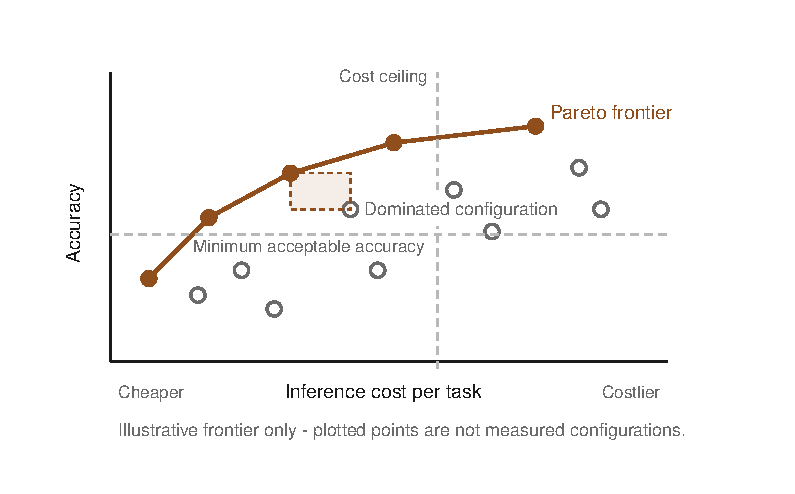
\includegraphics{figures/ch02-cost-accuracy-frontier.pdf}
\caption{Schematic of a cost-accuracy frontier, dominated configurations, and minimum-accuracy and cost-ceiling feasibility constraints.}
\end{figure}

Dominating configurations remove weaker alternatives unless an omitted property is measured separately. Deployment constraints then narrow the frontier.

The paired analysis from Chapter 1 keeps the frontier from acquiring false precision. Cost and accuracy estimates have uncertainty, and two nearby configurations may be indistinguishable at the available sample size. A single run also yields one realization of aggregate cost, which inherits the run-to-run variation that Chapter 1 describes for scores. The paired comparison runs on the per-task costs inside that run rather than on the aggregate. Preserve per-task cost as well as per-task correctness, so that bootstrap intervals can be computed for both axes and for the paired differences. A point should not be called cheaper or more accurate when the interval around that comparison does not support the ordering.

The retry arm needs the same accounting discipline as the candidate. If only some first attempts fail, report how often the second call fired, how much it cost when it fired, and whether it fixed the task. That record exposes the marginal value of the retry policy. A low-cost retry that recovers a meaningful subset of failures may dominate a planner with multiple unconditional calls, while a retry that repeats the same error adds cost without moving accuracy.

In CodeProbe, I report score per dollar alongside score and rank configurations by pass rate, cost, tokens, and latency. The end-to-end run in which the plain baseline led the tool-augmented arm on both axes came out of that report. It does not establish a general result about tools. Reporting both axes made the engineering decision visible without turning a small score difference into a claim about architecture.

Accuracy without a cost constraint still answers a legitimate research question. A model developer may want to know the highest capability reachable under extensive sampling, regardless of whether that procedure is economical in production. That is a capability probe. Selecting a system to operate under a budget is a different decision, and the result should state which decision the experiment was designed to support.

Architecture development introduces another source of optimism. An iteration \textbf{holdout} reserves a set of tasks that scaffold developers never use while choosing prompts, tools, routing rules, retry policies, or other configuration. Repeated iteration against a fixed evaluation set turns that set into training data for the scaffold, even when the model weights never change. Developers learn which changes improve the score, keep those changes, and discard the rest.

Create the iteration holdout before tuning begins. Use the remaining development tasks to debug the harness, compare early configurations, and decide what to carry forward. Open the iteration holdout only at a declared decision point, run the selected configurations, and do not use its task-level failures to continue tuning the same selection. If development resumes from those failures, the set has joined development and a new iteration holdout is needed.

The iteration holdout also needs protection from indirect tuning. A developer who reads its repository names, failure categories, or aggregate subgroup scores can adapt the scaffold to those features without inspecting the exact prompts. Access controls and an evaluation service that returns only the predeclared result can preserve the boundary better than a file accompanied by a policy. Record every opening, because repeated `final' checks use up the separation.

The cost of this discipline is fewer tasks for routine iteration. On small evaluations, that can reduce power enough to leave the final comparison inconclusive. The remedy is not to recycle the iteration holdout during development. Acquire more representative tasks, reduce the number of configurations carried into the final comparison, or accept a wider confidence interval. The boundary protects the interpretation of the result, but it does not add information the sample does not contain.

Search budget belongs in the accounting as well. If one architecture received hundreds of prompt and scaffold trials while the baseline received a single default configuration, the final inference-cost plot omits much of the effort spent finding the winner. Development cost and serving cost answer different questions. They should therefore be reported separately. At minimum, preserve the number of configurations tried, the selection rule, and the compute spent before the iteration holdout evaluation.

The companion catalog carries six related procedures. They cover expected best performance by tuning budget, repeated-sampling budgets based on coverage and verifier error, frozen-memory evaluation, a pinned scoring target, human-verified synthesis of evaluation instances, and baseline gates against random selection. Each refines a particular part of the experiment. None replaces the direct-call, retry, ablation, cost, and iteration-holdout controls developed here.

\hypertarget{build-the-next-comparison}{%
\section{Build the next comparison}\label{build-the-next-comparison}}

Start the next architecture comparison with the inexpensive arms. Run the base model directly, then run it with one retry under a failure signal the deployed system can observe. These controls establish how much of the candidate's accuracy another sample produces on its own, before a planner, memory writer, retriever, or second agent enters the design.

For each added component, create an arm without it and preserve every surrounding choice the design permits. When memory is the treatment, add raw-trajectory reuse so the experiment separates stored experience from the mechanism that rewrites it. When retrieval or tools are the treatment, add a no-tool arm, match task coverage, and record actual usage. Change one factor at a time unless the experiment is explicitly designed to estimate interactions.

Pilot the tasks before treating them as trials. Inspect each treatment trajectory and verify that the component entered the computation. A task the treatment never touches may measure general capability, cost, or incidental interference, but it decides nothing about the component's contribution. Remove it from that effect estimate under a rule declared in advance, or report it in a separate stratum.

Carry the per-task record from Chapter 1 into the cost analysis. For every arm, preserve correctness, input tokens, output tokens, priced cache quantities, call count, component usage, and wall-clock latency. Convert usage to dollars with a dated pricing snapshot. Plot accuracy against cost with confidence intervals, and prefer a configuration only when no cheaper configuration matches or exceeds its accuracy within the resolution of the evaluation.

Reserve the iteration holdout before the first scaffold change. Decide who can inspect it, when it can be opened, which aggregate results will be returned, and what event ends the comparison. Once developers have used its failures to revise the system, it has become development material. The boundary cannot be created retroactively around tasks the team has already learned to optimize.

\section*{Sources and evidence}

\textbf{Run ablation controls}

\begin{itemize}
\tightlist
\item
  Directional evidence: \emph{SkillEvolBench} (Lei et al.~2026, arXiv:2605.24117), through the agentic-memory source synthesis. The underlying study measures no-skill and raw-trajectory controls in its setting; coverage matching, one-factor sweeps, and the writer information-flow constraint are transfers within the broader protocol.
\item
  Directional evidence: evaluation-design material from the code-retrieval source corpus. CoIR (Li et al.~2024, arXiv:2407.02883) supplies code-retrieval tasks and metrics, but it does not test the no-tool baseline, tool-access control, or ground-truth-tautology checks recommended here.
\item
  Directional evidence: \emph{TIAP} (arXiv:2605.24060); no figure carried.
\item
  Directional evidence: \emph{MemConflict} (arXiv:2605.20926); no figure carried.
\item
  Strong evidence for the narrower transition analysis: Tank, D., and Nama, B. (2026), ``The Regression Tax: Decomposing Why Skills Help and Hurt LLM Agents,'' arXiv:2607.22520. Nearly 6,000 runs across two office-automation benchmarks and three model-harness stacks; transfer to coding-agent skill libraries is directional.
\end{itemize}

\textbf{Report cost-accuracy tradeoffs}

\begin{itemize}
\tightlist
\item
  Directional evidence: Kapoor, Stroebl, Siegel, Nadgir, and Narayanan (2024), \emph{AI Agents That Matter}, arXiv:2407.01502, a re-evaluation study.
\item
  Directional evidence: the iteration-holdout section rests on the same study, carried in the companion catalog as a separate record on holdout design split by generalization level.
\end{itemize}

\textbf{Author-system illustration cited inline}

\begin{itemize}
\tightlist
\item
  Not an evidence item: CodeProbe, the author's task-mining evaluation tool, \href{https://github.com/sjarmak/codeprobe}{public repository}. Named inline for the end-to-end run and the score-per-dollar reporting described above, both of which are narrative illustration.
\end{itemize}
